\chapter{MAC Protocols}

Duty cycle has a critical role for what concerns devices' networking. Turning the radio off on a device for some time ---indirectly--- affects also the other devices in the network, as they may not be able to communicate with the sleeping device.\\
It must be taken in consideration also that in low-powered multi-hop network, hence where only a few nodes have a direct connection to the access point, internal nodes may act as routers, and they may need to be awake to forward packets towards the access point.\\
In such scenario it is more clear why duty cycle and MAC protocols may disrupt performance and energy efficiency.

MAC protocols for IoT devices have some challenges, such as:
\begin{itemize}
   \item \textbf{Energy efficiency}: the protocol should be able to save energy, as the devices are battery-powered;
   \begin{itemize}
      \item Reduce duty cycle
      \item Maintain network connectivity
   \end{itemize}
   \item Find a \textbf{tradeoff} between Energy and Latency \& Bandwidth;
\end{itemize}
Three approaches are possible:
\begin{enumerate}
   \item \textbf{Synchronous MAC protocols} (\texttt{S-MAC}): nodes are synchronized and they know when to transmit and when to sleep;
   \item \textbf{Preamble sampling} (\texttt{B-MAC}): nodes wake up periodically to listen to the channel, and if they hear a preamble, they wake up completely to receive the packet;
   \item \textbf{Polling} (as in 802.15.4): a node is designated as the coordinator and it polls the other nodes to check if they have data to send.
\end{enumerate}

\section{Synchronization}
S-MAC is a protocol which implements only \textbf{local} synchronization.
It is based on the concept of \textit{periodic listening} and \textit{sleeping}; in fact, nodes alternate synchronized listen and sleep periods, i.e. they are all simultaneously active only for a short time. 

Synchronization is achieved by means of periodical (local)
broadcasts of SYNC frames containing the wake/sleep schedule of the node.
If a node detects adjacent nodes with a predefined schedule, it can synchronize with them, otherwise it chooses its own period, and broadcasts it with SYNC frames.
A node may revert its schedule to the one of other nodes in case it is not aligned with them

\subsection{Issues}
\begin{itemize}
   \item \textbf{Clock drift}: nodes may drift from their schedule, and they need to resynchronize;
   \note{Cheap IoT devices may have a clock drift of 1\% per day, and in general are considered to have an unreliable clock.}
   \item \textbf{Hidden terminal problem}: if a node is not synchronized with the others, it may transmit when it should not, causing collisions;
   \item \textbf{Overhead}: the SYNC frames may cause overhead, and they may not be received by all the nodes.
\end{itemize}

\textit{Adaptive listening} is a technique to reduce the overhead of SYNC frames, by making nodes listen for a longer time if they have not received a SYNC frame for a long time. This leads to slightly more energy consumption, but provides much better network performance, resulting in a good tradeoff.

S-MAC has \textit{never} been used as a standard, it relies on too many assumptions, and it is not suitable for large networks.

\section{Preamble Sampling}
In general we can measure the complexity of a solution to a problem in terms of how many parameters have to be tuned in order to make it work.
The more parameters, the more complex is to make it work, and the more likely it is to fail.
\begin{paracol}{2}
   
   B-MAC is extremely simple, and relies on the setup of a single parameter: the \textbf{wake-up interval}.
   A sender sends a packet \textbf{whenever} they want, but not \textit{whatever} they want:
   packets are sent with a \textit{long preamble} ---in other words, they start shouting before telling the actual information---, which is a sequence of bits that is sent before the actual packet, and it is used to wake up the receiver.\\
   Nodes activate their radio only for a short time to listen to a preamble, and if they hear one, they wake up completely to receive the subsequent packet.

   \switchcolumn
   
   \begin{figure}[htbp]
      \centering
      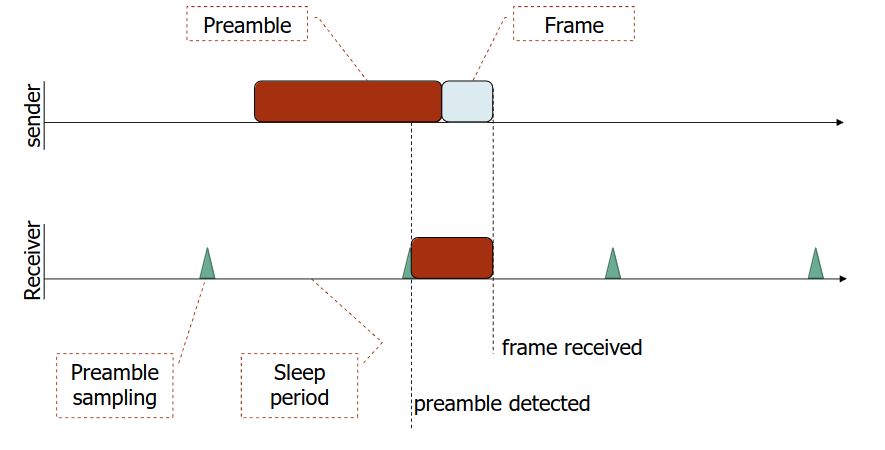
\includegraphics{images/BMAC.png}
      \caption{BMAC TX-RX schema}
      \label{fig:BMAC}
   \end{figure}
\end{paracol}

\begin{center}
   The key point is that \ul{the \textbf{preamble} should be longer than the \textbf{wake-up interval} (sleep period)}.
\end{center}
\note{This ensures that the receiver will not miss any packet preamble}

The idea is to waste some energy on the sender node in order to save energy on receiver ones.
Even though it appears slightly counterintuitive, it is a good tradeoff, because often there are more receivers than senders.

\note{The receiver has to stay awake ---on average--- for half the preamble, for the duration of the data transmission, and for the processing of such data. 
}
X-MAC is an improvement of B-MAC, which uses a \textbf{short preamble} to wake up the receiver, and then sends a \textbf{longer preamble} to synchronize with the receiver.
The preamble contains information about who should receive the data, and in case of BoX-MAC contains the data itself. The ``empty'' preamble is replaced by the repeated data interleaved with an ACK.  

\begin{figure}[htbp]
   \centering
   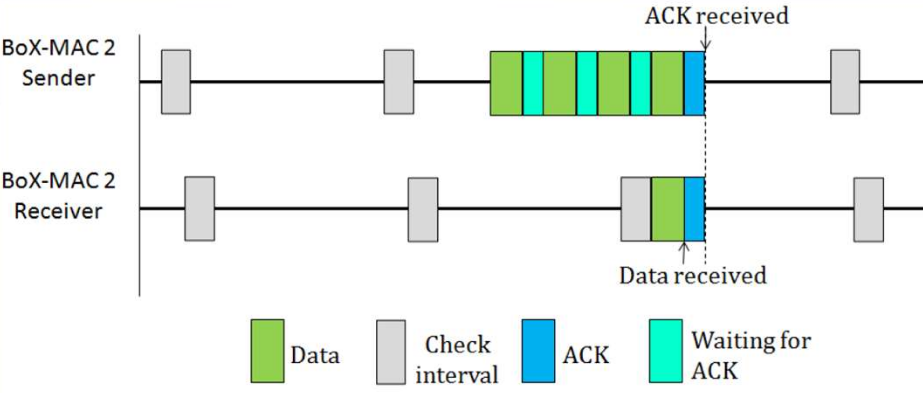
\includegraphics{images/BoXmac.png}
   \caption{BoX-MAC TX-RX schema}
   \label{fig:BoXmac}
\end{figure}

\section{Polling}
Polling is a technique used in 802.15.4, where the nodes are organized asymmetrically:
\begin{itemize}
   \item one master node issues periodic beacons
   \item several slave nodes that can keep the radio off whenever they want
\end{itemize}
When a slave hears the beacon and sees that there for pending messages for him, it requests them to the master.

\section{IEEE 802.15.4}

IEEE 802.15.4 is a standard specifying physical and MAC layers for low-rate wireless personal area networks (LR-WPANs).

It is infrastructure-less, short range and its Physical layer may coexist with IEEE 802.11 (Wi-Fi) and IEEE 802.15.1 (Bluetooth). 

\subsection{Physical Layer}

The Physical layer may operate in three possible frequency bands:
\begin{itemize}
   \item 868.3 MHz (Europe)
   \item 902-928 MHz (Americas) (11 channels, 2 MHz each)
   \item 2.4 GHz (Worldwide) (16 channels, 5 MHz each)
\end{itemize}

The Physical Layer works well even in low \textit{Signal-to-noise ratio} (\texttt{SNR}) environments, and it is able to work with a very low power consumption.
In other words, it is less likely to misread a packet.
\note{For example, the ``shouting'' of the preamble in B-MAC increases the SNR.}

\note{\begin{itemize}
   \item \textbf{Data Service}
   \begin{itemize}
      \item Transmission/Reception of PHY
      Protocol Data Unit (PPDU) through the physical
      medium.
   \end{itemize}
   
   \item \textbf{Management Service}
   \begin{itemize}
      \item Radio transceiver activation/deactivation (to
      implement policies of energy efficiency)
      \item Energy Detection - ED
      \item Link Quality Indicator – LQI
      \item Channel Selection
      \item Clear Channel Assessment – CCA
      \item PHY-PIB (PHY PAN Information Base) Configuration
   \end{itemize}
\end{itemize}}

\begin{figure}[htbp]
   \centering
   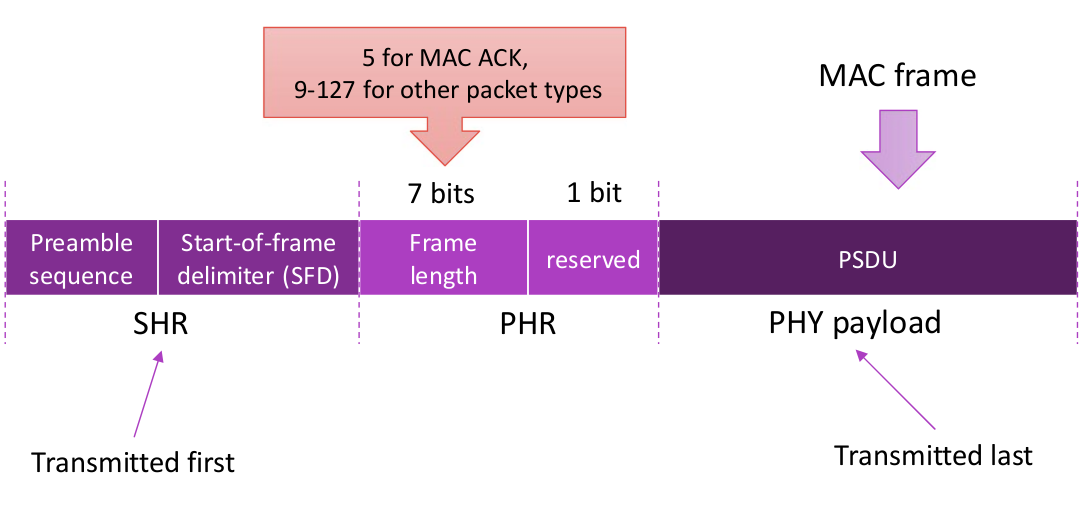
\includegraphics{images/802_physicalframe.png}
   \caption{Physical frame structure}
   \label{fig:802_physicalframe}

   \begin{itemize}
      \item \texttt{SHR} (Synchronization Header): synchronisation with the receiver
      \item \texttt{PHR} (PHY Header): information about the frame length
      \item \texttt{PHY} Payload: the MAC frame
   \end{itemize}
\end{figure}
   
\subsection{MAC Layer}

MAC layer provides various services:
\begin{itemize}
   \item \textbf{Data services}
   \begin{itemize}
      \item transmission and reception of MAC frames (MPDU)
      across the physical layer.
   \end{itemize}
   \item \textbf{Management services}
   \begin{itemize}
      \item Synchronization of the communications
      \item Channel access
      \item Management of guaranteed time slots
      \item Association and disassociation of devices.
   \end{itemize}
   \item \textbf{Security services}
   \begin{itemize}
      \item Data encryption
      \item Access control
      \item Frame integrity
      \item Sequential freshness
   \end{itemize}
\end{itemize}

This layer defined two types of devices:
\begin{itemize}
   \item \textbf{Full-function device} (FFD): can act as a coordinator;
   \item \textbf{Reduced-function device} (RFD): cannot act as a coordinator.
\end{itemize}


At the MAC layer there may be different network topologies:
\begin{itemize}
   \item \textbf{Star}: a central FFD PAN coordinator communicates with all the other nodes, which may be either FFDs or RFDs.
   \begin{figure}[htbp]
      \centering
      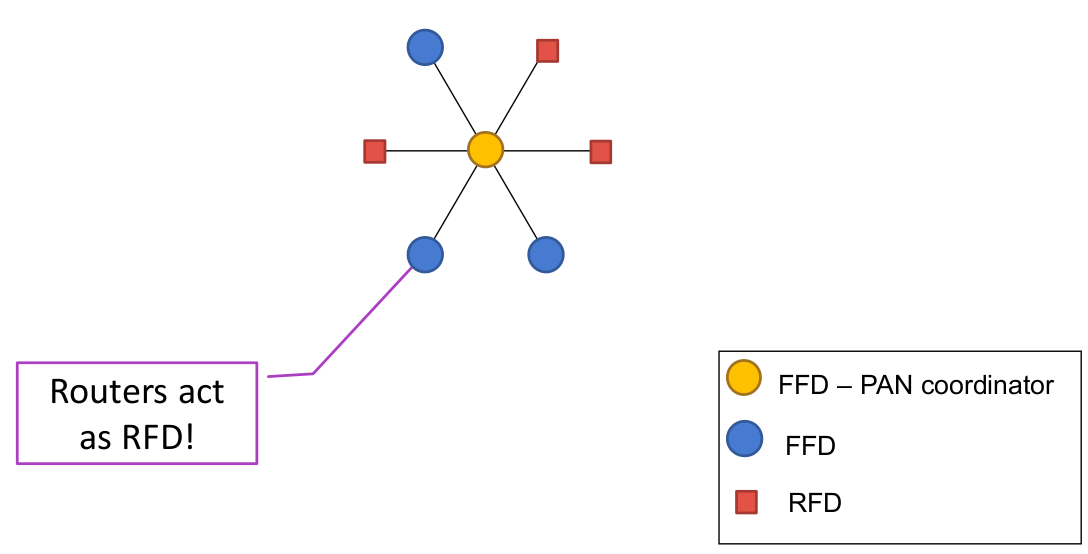
\includegraphics{images/802_star.png}
      \label{fig:802_star}
   \end{figure}
   \item \textbf{Peer-to-peer}: again there is a PAN coordinator, FFDs are routers and RFDs are end devices.
   \begin{figure}[htbp]
      \centering
      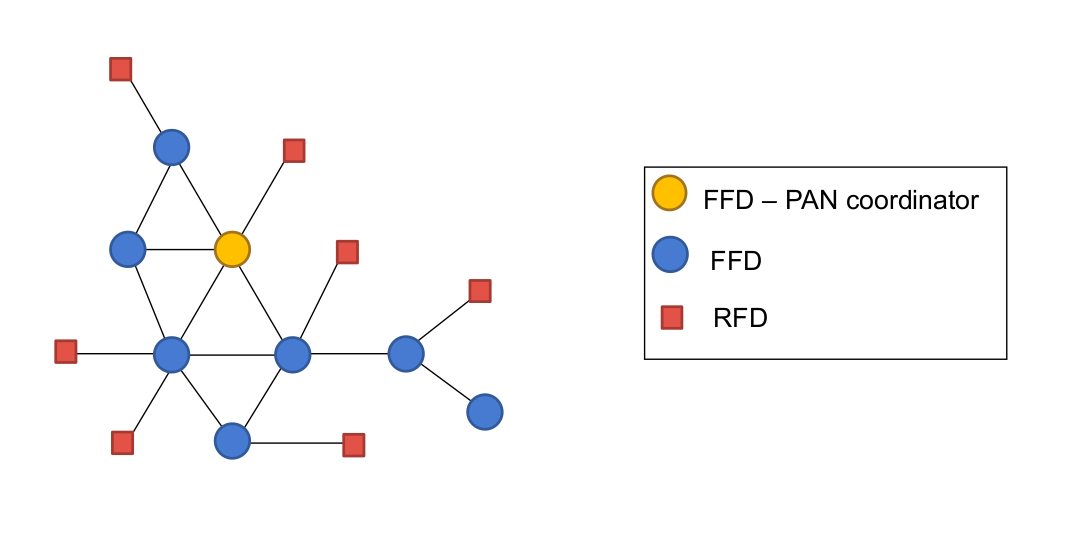
\includegraphics{images/802_p2p.png}
      \label{fig:802_p2p}
   \end{figure}
   \item \textbf{Cluster-tree}: a coordinator communicates with other coordinators, which in turn communicate with other nodes.